
% Change dir here
\def\covmac{/Users/matiascovarrubias/Documents/universidad/NYU/Research/Repositories/marketsAI/marketsai/Documents/Figures}
\let\dir=\covmac
%\documentclass[compress]{beamer} % notesonly

\documentclass[serif,9pt]{beamer}
%\documentclass[handout,9pt]{beamer} %use this to print 4 slides per page AND bibliography
%\usepackage{pgfpages}
%\pgfpagesuselayout{2 on 1}[letterpaper,border shrink=5mm]
%\documentclass[serif,notes]{beamer} %slides and notes interspersed
%\usepackage{pxfonts} % Or palatino or mathpazo
\usepackage{palatino}
%\usepackage{eulervm}
%\documentclass[handout]{beamer}
\usepackage{beamerthemesplit}
\usepackage{epsfig}
%\usepackage{pstricks,pst-plot}
\usepackage{mathpazo}
\usepackage{soul}
%\usepackage{epstopdf}
\usepackage{setspace}
\usepackage{hyperref}
\usepackage{graphicx}
\graphicspath{{Figures/}}
\usepackage{amsmath,amssymb}
\usepackage{spot}
%\usepackage[usenames,dvipsnames]{color}
\usepackage{tikz}
\usepackage{wasysym}
\usepackage{subcaption}
\newcommand{\pyobject}[1]{\fbox{\color{red}{\texttt{#1}}}}
\newcommand{\cmark}{\ding{51}}%
\usepackage[outdir=./]{epstopdf}
\newcommand{\rectangle}{\fboxsep0pt\fbox{\rule{1em}{0pt}\rule{0pt}{1ex}}}


% The following packages are from the file Tables.tex
\usepackage{float,graphicx}
\usepackage[justification=centering]{caption}
\usepackage{amsmath}
\usepackage{amssymb}
\usepackage{geometry}
\usepackage{color}
\newcommand\tsum{\textstyle\sum\nolimits}

\newcommand{\tlap}[1]{\raisebox{0pt}{#1}}
\newcommand{\myitem}[1]{\tlap{\rlap{\parbox[t]{\linewidth}{\item {\vspace{-2.2ex} \strut#1\strut}}}}}

%\usepackage[absolute,overlay]{textpos}
%\setlength{\TPHorizModule}{1mm}
%\setlength{\TPVertModule}{1mm}

%\usepackage{multirow}
% The following packages are from the file Tables.tex
%\usepackage{float,graphicx}
%\usepackage[justification=centering]{caption}
%\usepackage{amsmath}
%\usepackage{amssymb}
%\usepackage{geometry}
%\usepackage{color}
%\usepackage{subcaption}
%\usepackage{caption}
%\usepackage{hhline}
%\usepackage{arydshln}


%\usetheme{Antibes}
%\usetheme{Warsaw}
%\usetheme{Montpellier}
%\usetheme{Singapore}
%\usetheme{Szeged}
%\usetheme{Madrid}
%\usetheme{Darmstadt}
%\usetheme{Frankfurt}
%\usetheme{Berkeley}
\usetheme{CambridgeUS}
\usecolortheme{dolphin}

%If you use CabridgeUS theme, uncomment the lines below but above the ******* to control footnote, AND SET DATE BELOW
%\setbeamertemplate{footline}
%        {
%      \leavevmode%
%      \hbox{%
%      \begin{beamercolorbox}[wd=.333333\paperwidth,ht=2.25ex,dp=1ex,center]{author in head/foot}%
%        \usebeamerfont{author in head/foot}\insertshortauthor%~~(\insertshortinstitute)
%      \end{beamercolorbox}%
%      \begin{beamercolorbox}[wd=.333333\paperwidth,ht=2.25ex,dp=1ex,center]{title in head/foot}%
%        \usebeamerfont{title in head/foot}\insertshorttitle
%      \end{beamercolorbox}%
%      \begin{beamercolorbox}[wd=.333333\paperwidth,ht=2.25ex,dp=1ex,right]{date in head/foot}%
%        \usebeamerfont{date in head/foot}\insertshortdate %\hspace*{2em}
%      \end{beamercolorbox}}%
%      \vskip0pt%
%    }
%END CAMBRIDGE US THEME MODIFICATIONS***********************************************************************************************

%\setbeameroption{show only notes}

%\usepackage{etoolbox}
%\patchcmd{\quote}{\rightmargin}{\leftmargin 1em \rightmargin}{}{}
\newenvironment{myquote}{\list{} {\leftmargin=0.0in\rightmargin=0.3in \scriptsize \itshape }{}\item[]}{\endlist}

\newtheorem{prop}{Proposition}
\newtheorem{proposition}[theorem]{Proposition}

\newcommand{\ra}{$\rightarrow \hspace{0.1cm}$}
\newcommand{\Ra}{$\Rightarrow \hspace{0.1cm}$}
\newcommand{\Ua}{$\Uparrow \hspace{0.1cm}$}
\newcommand{\Da}{$\Downarrow \hspace{0.1cm}$}

\newcommand{\be}{\begin{equation}}
	\newcommand{\ee}{\end{equation}}
\newcommand{\bes}{\begin{equation*}}
	\newcommand{\ees}{\end{equation*}}
\newcommand{\bi}{\begin{itemize}}
	\newcommand{\ei}{\end{itemize}}
\newcommand{\ms}{\medskip}
\newcommand{\bs}{\bigskip}
\newcommand{\sms}{\smallskip}

\newcommand{\mhat}{\hat{\mu}}
\newcommand{\hmu}{\hat{\mu}}
\newcommand{\ahat}{\hat{a}}
\newcommand{\sa}{\sigma_a}
\newcommand{\si}{\sigma_i}
\newcommand{\sx}{\sigma_x}
\newcommand{\ha}{\hat{a}}
\newcommand{\shata}{\hat{\sigma}_a}
\newcommand{\hi}{\hat{s}_i}
\newcommand{\shati}{\hat{\sigma}_i}
\newcommand{\shat}{\hat{\sigma}}
\newcommand{\Shat}{\hat{\Sigma}}
\newcommand{\sna}{\sigma_{\eta a}}
\newcommand{\sno}{\sigma_{\eta 1}}
\newcommand{\snt}{\sigma_{\eta 2}}
\newcommand{\ex}{\bar{x}}
\newcommand{\epsi}{\varepsilon}
\newcommand{\p}[1]{\left( #1 \right)}
\newcommand{\h}{\mathcal{H}}
\newcommand{\M}{\mathcal{M}}
\newcommand{\E}{\mathbb{E}}
\newcommand{\V}{\mathcal{V}}
\newcommand{\La}{\mathcal{L}}
\newcommand{\W}{\mathcal{W}}
\newcommand{\T}{\mathbb{T}}
\newcommand{\dom}{\mathcal{D}}
\newcommand{\pc}{\perp_C}
\newcommand{\vecspan}{\operatorname{span}}
\newcommand{\interior}{\operatorname{int}}
\newcommand{\lcm}{\operatorname{lcm}}
\newcommand{\tr}{\operatorname{tr}}
\newcommand{\divides}{|}
\newcommand{\claim}{Claim: }
\newcommand{\tmu}{\tilde{\mu}}
\newcommand{\wt}[1]{\widetilde{#1}}
\newcommand{\wb}[1]{\overline{#1}}
\newcommand{\wh}[1]{\widehat{#1}}
\newcommand{\pare}[1]{\left( #1 \right)}

\newcommand\smallfont{ \usefont{T1}{ptm}{m}{n}\fontsize{9pt}{9pt}\selectfont\DB}
\newcommand\verysmallfont{\usefont{T1}{ptm}{m}{n}\fontsize{8pt}{8pt}\selectfont}%
\renewcommand{\cite}{\citeasnoun}
\renewcommand<>{\sout}[1]{\alt#2{\beameroriginal{\sout}{#1}}{#1}}
\def\DPbar{\overline{DP}}

%\newrgbcolor{LG}{0.91 0.91 0.91}
%\newrgbcolor{DB}{0.00 0.00 0.6}
%\newrgbcolor{DR}{0.503 0 0}
%\newrgbcolor{OR}{1.00 0.35 0.00}
%\newrgbcolor{dgreen}{0.00 .50 .00}
\newtheorem{result}[theorem]{Result}

%\definecolor{green}{RGB}{0 100 0}
\definecolor{green}{RGB}{0 200 0}
\definecolor{purple}{RGB}{138 	43 	226 	}
\definecolor{limegreen}{RGB}{50 205 50}

\usepackage{tikz}
\usetikzlibrary{shapes}
\usetikzlibrary{fadings}

%% For rectangles %% lines below for blue rectangles
%\tikzfading[name=spotfade2,
%% inner color=transparent!100,
% %outer color=transparent!90]
% inner color=transparent!200,
% outer color=transparent!80]
%\definecolor{colorspot}{RGB}{0 	255  255}

% For rectangles %% lines below for yellow rectangles
\tikzfading[name=spotfade2,
inner color=transparent!100,
outer color=transparent!20]
\definecolor{colorspot}{RGB}{    255  255 0}


% For the remaining spotlights
\tikzfading[name=spotfade,
inner color=transparent!100,
outer color=transparent!80]

\setspotlightstyle{ball color=cyan,fill=cyan, path fading=spotfade, draw=cyan, thick }%
%,fill opacity=0.1


\title{\textbf{MarketsAI}}
\subtitle{A Deep Reinforcement Learning Approach to Simulate High-Dimentional and Imperefect Information Economies}
\author[Covarrubias]
{Matias Covarrubias}
\institute[NYU]{NYU}

%\date[December 2011]{}
\date[]{}

\setbeamertemplate{navigation symbols}{}

\begin{document}
\begin{frame}
  \titlepage
\end{frame}

\section{Introduction}
%%% SLIDE 1 %%%
\begin{frame}
\frametitle{Motivation: Deep RL as an implementation of Rational Expectations}

 I borrow two elements from modern AI literature: \ms
	
	\begin{enumerate}
		\item Agents use Reinforcement Learning (RL) to choose actions.\ms
		
		\begin{itemize}
			\item On simple environments, agent behavior is consistent with Rational Expectation.  \ms
			
			\item They learn by interacting with environment. No need to find explicit fixed point between expectations and policies $\to$ computationally tractable. \ms
			
			\item We only need to characterize their environments and simulate interactions $\to$ easy to program.  \ms
		\end{itemize}
	
		\item Agent-environment separation. Households and Firms are agents. Markets are environments. Advantages: \ms
		
		\begin{itemize}
			
			\item Scalability: Many techniques to increase scale of models. \ms
			
			\item Modularity: This allow us to construct economies combining pre-specified agent and environment modules. \ms
			

		\end{itemize}
	\end{enumerate}
\end{frame}

\begin{frame}
\frametitle{Agenda}


\begin{enumerate}
	\item Centralized planing problem.\ms
	
	
	\begin{itemize}
		\item Can be formalized as a Markov Decision Problem $\to$ theoretical guarantees.  \ms
		
		\item \textbf{Benchmark}. Stochastic Growth model plus investment adjustment costs. \ms
		
	\end{itemize}
	
	\item Decentralized (multi-agent) problems. \ms
	
	\begin{itemize}
		
		\item Can be formalized as Partially Observed Markov Games $\to$ few theoretical guarantees. \ms
		
		\item Challenge: non-stationarity. Agents learn while others are learning (and experimenting) as well. \ms
		
		\item \textbf{Benchmark}. Durable good market.
	\end{itemize}

	\item Large-scale problems \ms

\begin{itemize}
	
	\item Many heterogeneous agents. \textbf{Benchmark}: Krussel-Smith (1998).  \ms
	
	\item Many markets.  \textbf{Application}: Capital Goods Supply and Boom and Bust Dynamics.
	
\end{itemize}

\end{enumerate}

\end{frame}

\begin{frame}
\frametitle{The learning workflow}
\begin{figure}
	\centering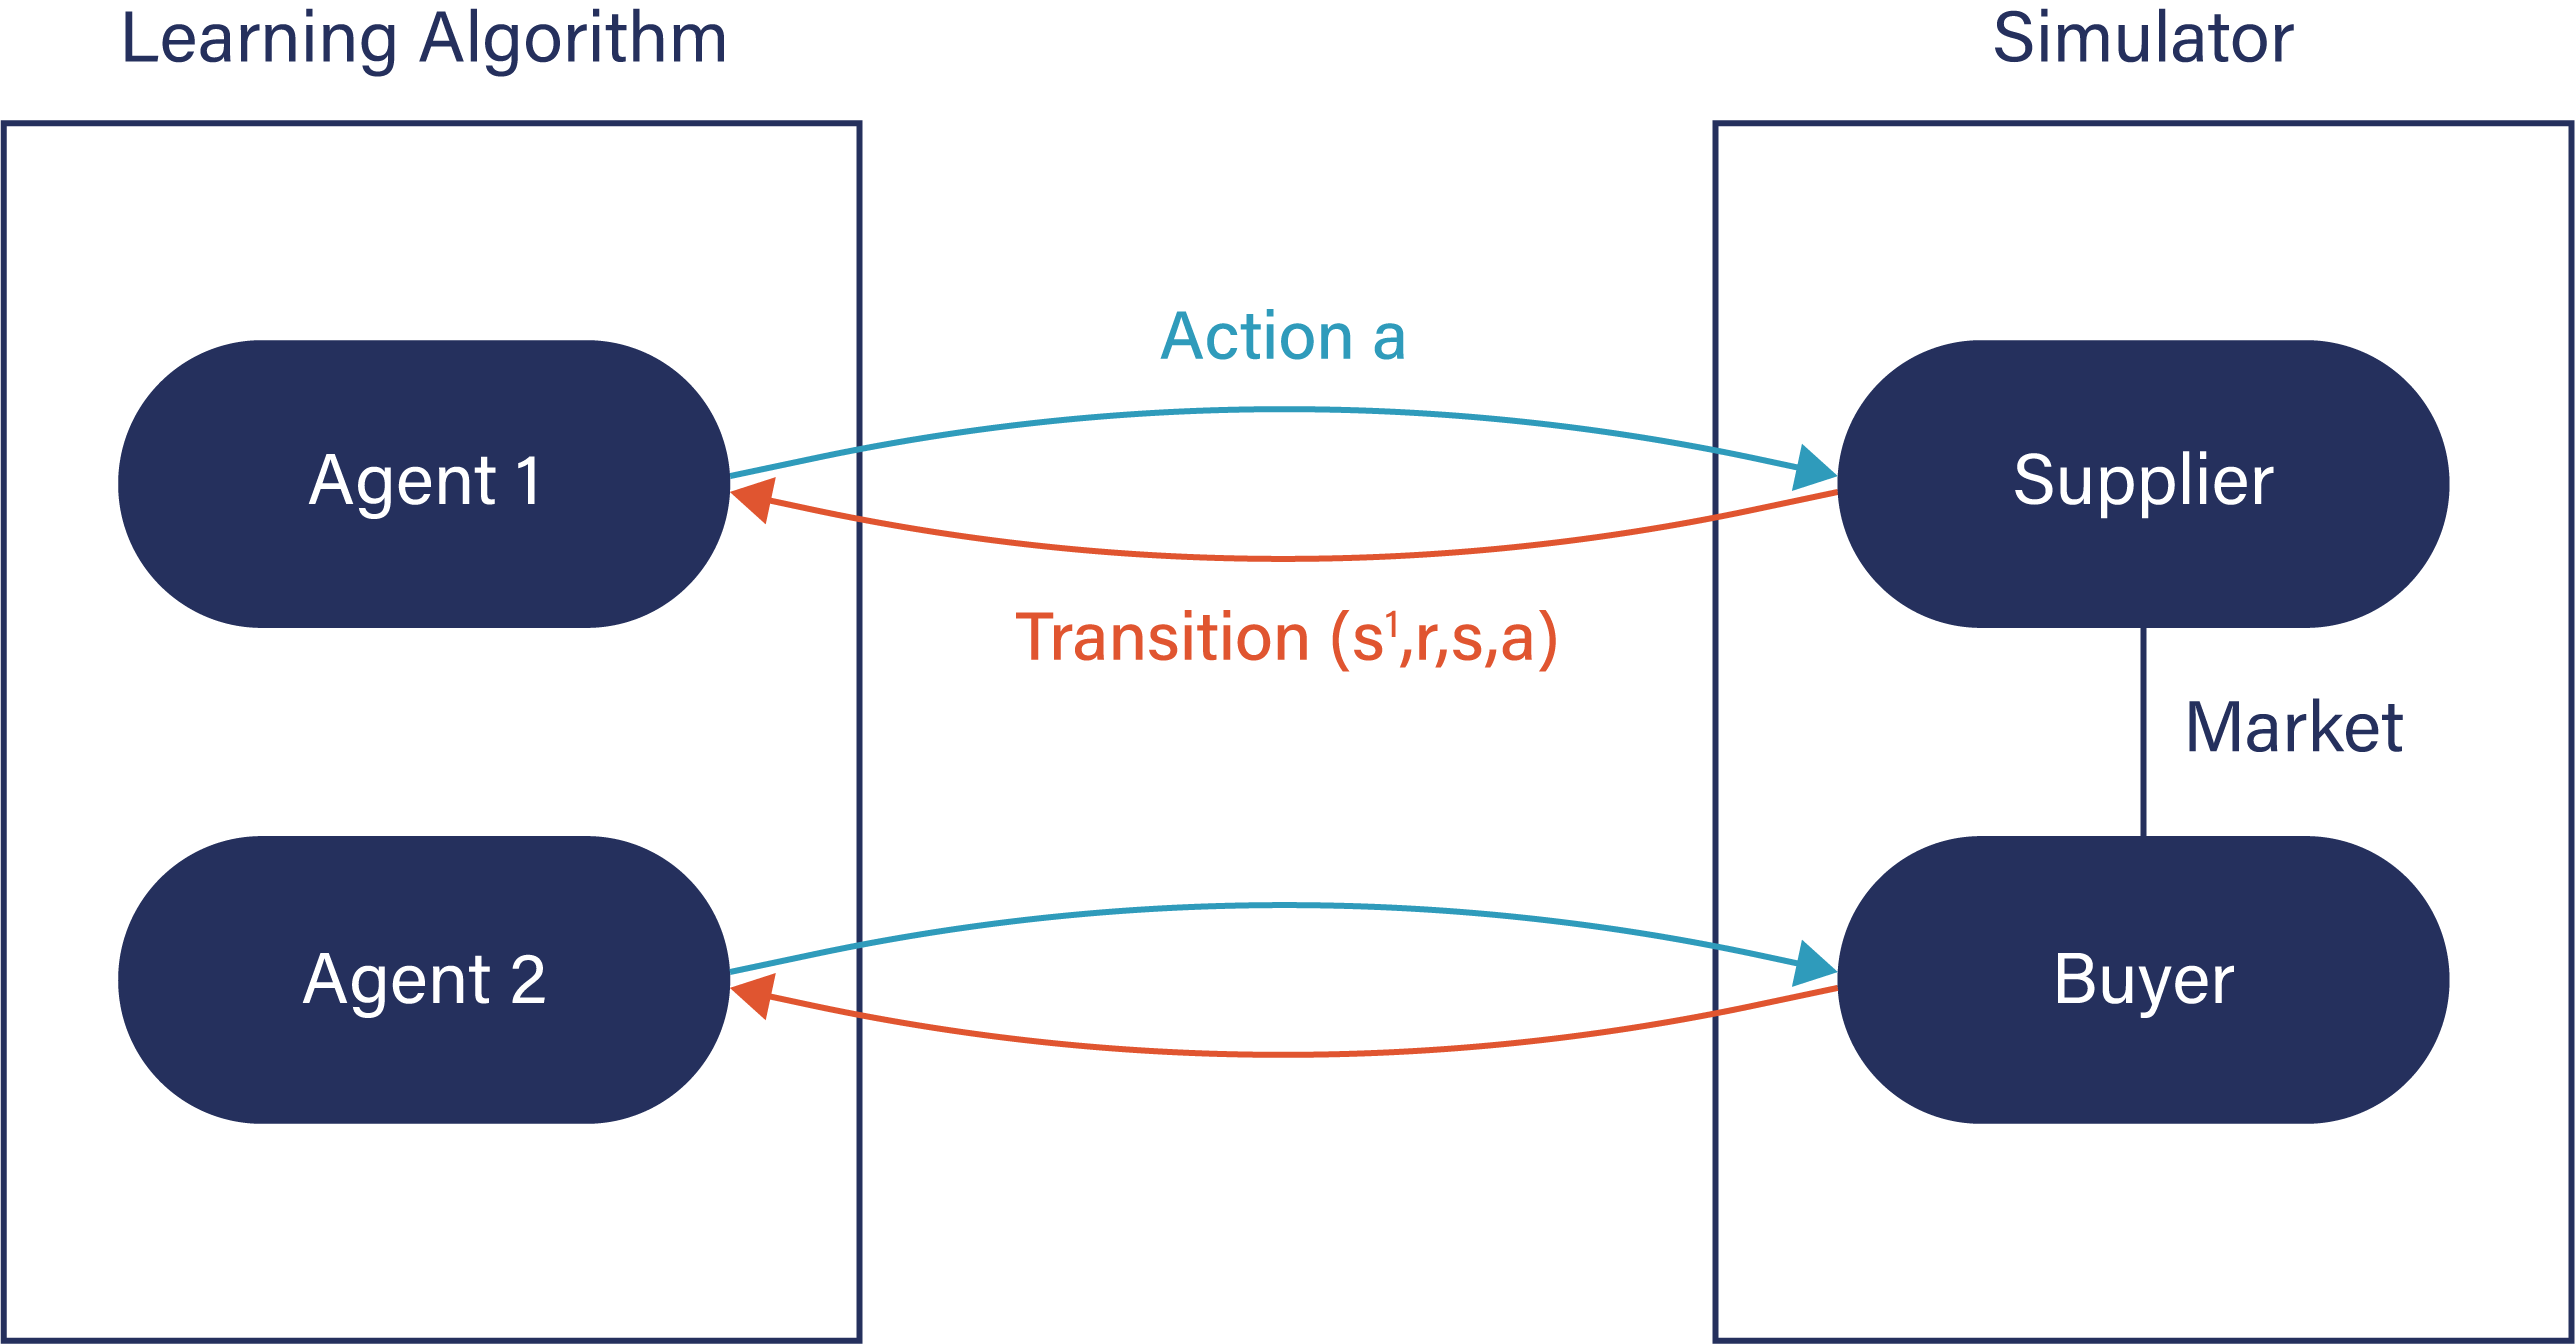
\includegraphics[scale=0.2]{\dir/Online-learning.png}
	\caption{Online learning workflow}
\end{figure}
\end{frame}

%%% SLIDE 5 %%%

%%% SLIDE 2 %%%
\begin{frame}
\frametitle{Formalizing the Simulator}

We formalize an economy as a a Partially Observed Markov Game. In each period:\medskip

\begin{itemize}
	\item $n$ agents indexed by $i$ choose an action $a_i \in \mathcal{A}_i$, after observing a state $s_i \in \mathcal{S}_i $. \medskip
	
	\item Let $\mathcal{S}$ be set of states, that is, the collection of all possible states $S_i$. \ms 
	
	\item The initial states are determined by a distribution $\rho:\mathcal{S} \mapsto [0,1]$.\medskip
	
	\item To choose actions, each agent $i$ uses a stochastic policy $\pi_{\theta_i}: \mathcal{S}_i \times \mathcal{A}_i \mapsto [0,1]$. \ms
	
	\item The combined actions produces the next state according to the state transition function $p:\mathcal{S} \times \mathcal{A}_i \times ... \times \mathcal{A}_N \mapsto \mathcal{S}$. \medskip
	
	\item Each agent $i$ observes its reward as a function of the state and agent's action $r_i:\mathcal{S} \times  \mathcal{A}_i \times ... \times \mathcal{A}_N \mapsto \mathcal{R}$, and receives a private observation  $s'_i: \mathcal{S} \mapsto \mathcal{S}_i$.  \medskip
	
	
\end{itemize}
\end{frame}

\section{Single-Agent}
%%% SLIDE 2 %%%
\begin{frame}
\frametitle{Our first environment}

\begin{itemize}
	\item A representative household chooses how much to consume and how much to invest in order to maximize $\sum_{t=0}^{\infty} \beta^t u(c_t)$.\ms
	

	\begin{align*}
	V_t\left(k_t\right) = &\max_{s_t} U(c_t) + \E_t M_{t,t+1}V_{t+1}(k_{t+1}) \qquad \text{s.t.}\\
	&\qquad
	c_t = y_t(1-s_t) \\
	&\qquad
	y_t = k_t^\alpha\\
	&\qquad
	K_{t+1} = (1-\delta) K_t + s_t y_t 
	\end{align*}
	
	where: \ms

	\item Utility from consumption: $U(c_t) = \frac{C^(1-\gamma)}{1-\gamma}+1$. \ms
	
	\item Production function: $f(k_t) = \theta k_t^{\alpha}$. \ms
	
	
	\item Evolution of capital: $k_{t_1}=(1-\delta)k_t + i_t$. \ms

\end{itemize}
\end{frame}

\section{Single-Agent}
%%% SLIDE 2 %%%
\begin{frame}
\frametitle{We add uncertainty}

\begin{itemize}
	\item A representative household chooses how much to consume and how much to invest in order to maximize $\sum_{t=0}^{\infty} \beta^t u(c_t)$.\ms
	
	
	\begin{align*}
	V_t\left(k_t\right) = &\max_{s_t} U(C_t) + \E_t M_{t,t+1}V_{t+1}(k_{t+1}) \qquad \text{s.t.}\\
	&\qquad
	c_t = y_t(1-s_t) \\
	&\qquad
	y_t = {\color{blue}\theta}  k_t^\alpha\\
	&\qquad
	K_{t+1} = (1-\delta) K_t + s_t y_t 
	\end{align*}
	
	where:
	
	\item Utility from consumption: $U(c_t) = \frac{C^(1-\gamma)}{1-\gamma}+1$. \ms
	
	\item Production function: $f(k_t) = {\color{blue}\theta} k_t^{\alpha}$. \ms
	
	\item Evolution of capital: $k_{t_1}=(1-\delta)k_t + s_t y_t$. \ms
	
	\item {\color{blue} Productivity $\theta$ follows a two-state markov process with transition probability $\mathcal{P}$.} \ms
	
\end{itemize}

\end{frame}

\begin{frame}
\frametitle{We add convex adjustment costs}
\begin{itemize}
	\item A representative household chooses how much to consume and how much to invest in order to maximize $\sum_{t=0}^{\infty} \beta^t u(c_t)$.\ms
	
	\begin{align*}
	V_t\left(k_t\right) = &\max_{s_t} U(C_t) + \E_t M_{t,t+1}V_{t+1}(k_{t+1}) \qquad \text{s.t.}\\
	&\qquad
	c_t + {\color{blue}\phi (\frac{i}{k})^2 k }= y_t(1-s_t) \\
	&\qquad
	y_t = \theta  k_t^\alpha\\
	&\qquad
	K_{t+1} = (1-\delta) K_t + s_t y_t 
	\end{align*}
	
	where:
	
	\item Utility from consumption: $U(c_t) = \frac{C^(1-\gamma)}{1-\gamma}+1$. \ms
	
	\item Production function: $f(k_t) =\theta k_t^{\alpha}$. \ms
	
	\item Evolution of capital: $k_{t_1}=(1-\delta)k_t + s_t y_t$. \ms
	
	\item  Productivity $\theta$ follows a two-state markov process with transition probability $\mathcal{P}$. \ms
	
	\item {\color{blue}Convex adjustment cost: $C(\frac{i}{k})=\phi (\frac{i}{k})^2 k$. }\ms
\end{itemize}
\end{frame}

\begin{frame}
\frametitle{Results for determistic case}
\begin{figure}
	\centering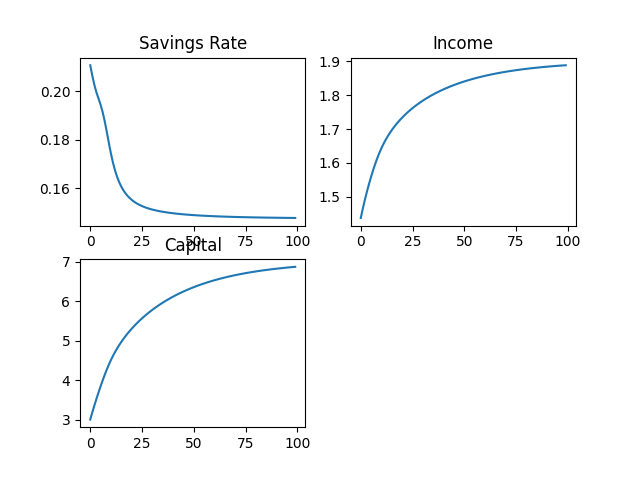
\includegraphics[scale=0.6]{\dir/sgm_IR_PPO_June11_big.png}
\end{figure}
\end{frame}

\begin{frame}
\frametitle{Results for stochastic case}
\begin{figure}
	\centering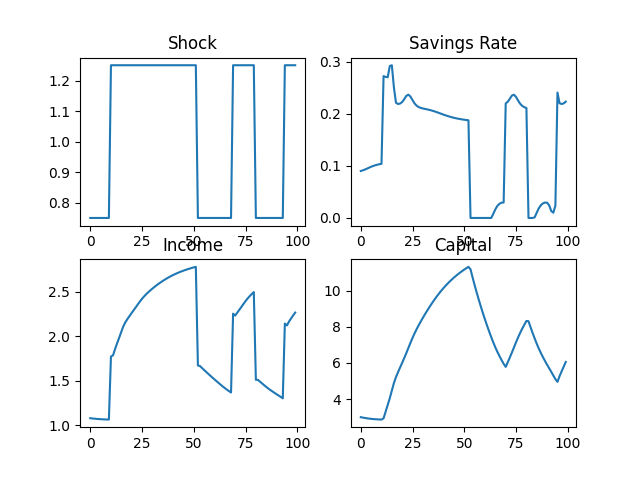
\includegraphics[scale=0.6]{\dir/stoch_IR_PPO_June11_big.png}
\end{figure}
\end{frame}

\begin{frame}
\frametitle{Results for adjustment cost case case}
\begin{figure}
	\centering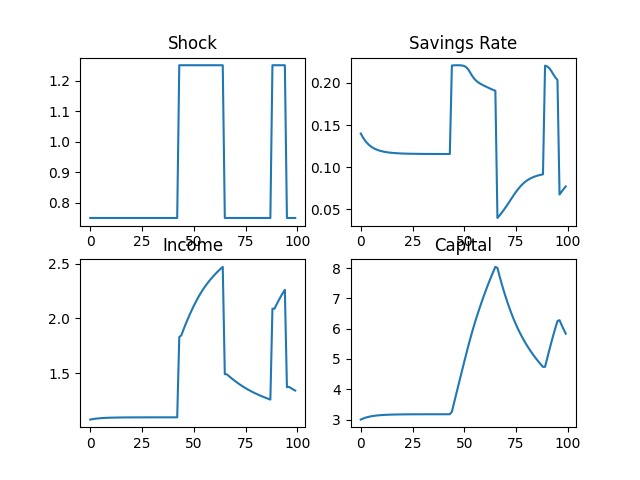
\includegraphics[scale=0.6]{\dir/adj_IR_PPO_June11_big.png}
\end{figure}
\end{frame}

\begin{frame}
\frametitle{Endogenous Time-to-Build}
\begin{itemize}
	\item The problem is the same as before but with with an inventory process for investment and an expanded action space. \ms
	
	\item There  are$N^{TTB}$ stages (we index them from 0 to$ N^{TTB}-1$). The agent decides the scale of the new projects and the progress of the projects through the stages. \ms
	
	\item New projects go directly to stage $0$. Then, for each stage, the agent decides what percentage to move 1 stage ahead ($z_{i,i+1}$ for $i \in [0,..,N^{TTB}-1]$) and what percentage to move 2 stages ahead $z_{i,i+2}$ for $i \in [0,..,N^{TTB}-2]$). \ms
	
	\item The rest ($1-z_{i,i+1}-z_{i,i+2}$) stays in the stage $i$. We have $N^{TTB}-1$ occasionally binding constraints $z_{i,i+1}+z_{i,i+2}<1$. \ms
	
	\item The state space now includes $\{K_t, \theta_t, \{x_{i,t}\}_{i \in [0,..,N^{TTB}-1]} \}$ where $x_{i,t}$ is the stock of projects at stage $i$ at time $t$. \ms
\end{itemize}
\end{frame}

\begin{frame}
\frametitle{Endogenous Time-to-Build}
\begin{itemize}
	\item The cost of progressing through stages is increasing in speed. \ms
	
	\item Each stage represents a proportion $\omega_i$ of the total cost and $\sum_{i=0}^{N^{TTB}-1}=1$. if you move one unit of capital that its at stage $i$ two stages ahead, you pay $(\omega_{i+1}+\omega_{i+2}) \phi$, where $\phi$ is the speed penalty. \ms
	
	\item There is also a convex adjustment cost over $Z_t$,  the total investment spending, which is the sum of the progress spending of each stage: $C(Z)=\psi (\frac{Z}{2})^2 k_t$ .
	
	\item The evolution of capital is $$k_{t+1} = (1-\delta)k_t + z_{N^{TTB}-1,N^{TTB}}+z_{N^{TTB}-2,N^{TTB}}$$. \ms
\end{itemize}
\end{frame}

\section{Multi-Agent}

\begin{frame}
\frametitle{Market: Durable Good supplied elastically}

\begin{itemize}
	\item Agents: $n^s>=1$ suppliers.  $n^b>=1$ buyers. \ms
	\item Action space:  \ms
	\begin{itemize}
		\item Supplier: Each supplier chooses a price $p'_i \in \mathbb{R}$ for the next period. \ms
		\item Households: each buyer chooses a quantity vector $h_i \in \mathbb{R}^{n^s}$. \ms
	\end{itemize}
	
	
	\item State space: The state space of all agents include: \ms
	\begin{itemize}
		\item  The current price vector ($\mathbf{p}$), chosen the previous period. \ms
		\item The stock of good $j$ owned by agent $i$: $\{H^j_i\}_{i,j}$.   \ms
		\item Stochastic parameters (e.g., depreciation shock for each good). \ms
	\end{itemize}
	
	
\end{itemize}

\end{frame}

\begin{frame}
\frametitle{Market: Durable Good supplied elastically}

\begin{itemize}

	\item Step \pyobject{s', R = step(p',h)}: 
	
	\begin{align*}
	R_j^s & = (p_j-c_j) \sum_{j=1}^{n^b} h_i^j  \\
	R_i^b  & = U_i({H^j_i}) +\mu_i \mathbb{1}(I_i<\sum_{j=1}^{n^s} h_i^j p_j) \\
	{H_i^{j}}' &=(1-\delta_j)H_i^j+h_i^j\\
	s' &  =  \{p', \{{H_i^{j}}'\}_i  \}  
	\end{align*}
	
	where $h_i^j$ is the demand of agent $i$ of product $j$ and $\delta_j$ is the depreciation rate of good $j$ \ms
\end{itemize}

\end{frame}

\begin{frame}
\frametitle{Decentralized markets: Durable Good supplied inelastically}

\begin{itemize}
	\item Agents: $n^s>=1$ suppliers.  $n^b>=1$ buyers. \ms
	\item Action space:  \ms
	\begin{itemize}
		\item Suppliers: Each supplier chooses a price $p'_j \in \mathbb{R}$ and quantity $\tilde{h}^s_{j}$ to develop for the next period. \ms
		\item Buyers: each buyer chooses their intended quantity $\hat{h}^j_i$ give prices. This will not necessarily correspond to the obtained quantity $h_i^j$, since the inventory needs to be allocated. \ms
	\end{itemize}
	
	
	\item The state space of all agents include: \ms
	\begin{itemize}
		\item  The current price vector ($\mathbf{p}$), chosen the previous period. \ms
		\item Each buyer $i$ observes his stocks of good $j$. Each supplier $j$ knows the stock of his good owned by each buyer $i$.   \ms
		\item The inventory of good $j$ available for selling: $\{h^s_j\}_j$. \ms
		\item Stochastic parameters (e.g., depreciation shock for each good). \ms
	\end{itemize}
\end{itemize}

\end{frame}

\begin{frame}
\frametitle{Market: Durable Good supplied inelastically}

\begin{itemize}

\item Step \pyobject{s', R = step(p)}: 

\begin{align*}
h_i^j  & =f(\{\hat{h}^j_i \}_i,h^s_j) \\
R_j^s & = p_j \sum_{j=1}^{n^b} h_i^j -C_j({\tilde{h}^s}_j)  \\
R_i^b  & = U({H^j_i}) +\mu_i \mathbb{1}(I_i<\sum_{j=1}^{n^s} h_i^j p_j) \\
{H_i^{j}}' &=(1-\delta_j)H_i^j+h_i^j\\
{h^{s}_j}' &=\tilde{h}^s_{j}+h^s_j-\sum_{j=1}^{n^b} h_i^j \\
s' &  =  \{p', \{{H_i^{j}}'\}_i, \{{h^{s}_j}'\}_i  \} 
\end{align*}

where $h_i^j$ is realized quantity obtained by buyer $i$ of product $j$. \ms
\end{itemize}

\end{frame}




%%% SLIDE 11 %%%

\begin{frame}
\frametitle{Reinforcement Learning: Overview}

\begin{itemize}
	\item We start from simplest single agent algorithm. The problem is: \ms
	$$\underset{a \in A}{\max} \sum_{t=s}^{\infty} \gamma^{s-t} E_t[r_{t+s}]$$
	
	\item Two value functions:\ms
	\begin{enumerate}
		\item state-value function: $V(s)=\max_{a\in A} \{E[r|s,a] + \gamma E[V(s')|s,a] \}$ \medskip
		\item action-value function: $Q(s,a)=E(r|s,a)+\gamma E[\max_{a'\in A} Q(s',a')|s,a]$ \medskip
	\end{enumerate}
	\item Q-Learning: \ms
	\begin{itemize}
		\item Initialize $Q_0(s,a)$. Loop until converge: \ms
		\begin{itemize}
			\item agent chooses $a= \text{arg} \max Q(s,a)$  and observes $\{r, s'  ,s, a\}$. \ms
			\item Old Q: $Q(s,a)$. \ms
			\item  Target Q: $r_t+\gamma \max_{a' \in A} Q(s',a')$. \ms
			\item New Q: $$Q'(s,a)=(1-\alpha) Q(s,a) +\alpha [r+\gamma \max_{a' \in A} Q(s',a')]$$ \ms
		\end{itemize}
	\end{itemize}
\end{itemize}

\end{frame}

%%% SLIDE 3 %%%
\begin{frame}
\frametitle{Getting deeper: Deep RL}

\begin{itemize}
\item Deep Q-learning consists in approximating the Q function with a neural net: $\hat{Q}(s,a) \equiv  \mathcal{N}_\rho \sim Q(s,a)$.\ms
\item The parameters $\rho$ are estimated in order to minimize \ms
$$\mathcal{L}(\rho)=\E \left[ \left(\hat{Q}(s,a)-(r_t+\gamma \max_{a' \in A} \hat{Q}(s',a')) \right)^2 \right] $$

in observed transitions $\{r, s'  ,s, a\}$ .\ms

\item A common example of a NN is a composite function made of nested linear functions:  \ms

$$\mathcal{N}_\rho (x)=\sigma_K(W_K ... \sigma_2(W_2 \sigma_1(W_1x+b_1)+b_2)...+b_K)$$

where $x$ is the input (in our case the transitions $\{r, s'  ,s, a\}$), $W_i \in \mathbb{R}^{m_{i+1}\times m_i}$ are the weights, $b_i \in \mathbb{R}^{m_i+1}$ are the biases, and $\sigma()$ are activation functions.
\end{itemize}

\end{frame}

\begin{frame}
\frametitle{Convergence results in RL}


\begin{itemize}
\item  Tsitsiklis (1994) If state space and action space are discrete, Q-learning converges globally if: \ms
\begin{itemize}
\item All state-action pairs are visited infinitely often. \ms
\item Conditions on learning rate $\alpha$. The sum $\sum_{t=0}^{\infty} \alpha_t^2$ is finite and $\sum_{t=0}^{\infty} \alpha_t$ is infinite. \ms
\end{itemize}

\item Tsitsikli and Van Roy (1997) prove convergences in the case of linear function approximators and Maei et al (2009) prove convergence with smooth non-linear approximators (e.g., neural nets). \ms

\item For multi-agent, convergence is hard to prove. Muller et al (2019) show convergence in a large class of games to a solution concept they called $\alpha$-rank.
\end{itemize}


\end{frame}



\begin{frame}
\frametitle{Taxonomy of State of the Art Algorithms}

There are three objects that the agents can learn:


\begin{enumerate}
\item q function $Q(s,a)$ \ms
\begin{itemize}
\item \textbf{Q-based methods} use NNs to represent $Q(s,a)$.  \ms
\item off-policy method: the NN can learn from steps taken by any policy.  \ms
\item Model-free method.  \ms
\end{itemize}

\item policy function $\pi(s,a)$  \ms
\begin{itemize}
\item \textbf{Policy-gradient methods} use NN to represent $\pi(s,a)$.  \ms
\item on-policy method. the NN only learns from steps taken from optimal policy.  \ms
\item Model-free. More stable than $Q$ but less sample efficient.  \ms
\end{itemize}

\item Model $p(r,s'|s,a)$  \ms
\begin{itemize}
\item \textbf{Model-based methods} uses different methods to represent $p(r,s'|s,a)$.  \ms
\item In recent stage of development compared to other methods.  \ms
\end{itemize}
\end{enumerate}

\end{frame}


\begin{frame}
\frametitle{In practice: How to create environments and agents}

An environment consists of a \textbf{reset} and a \textbf{step} function. \ms

An agent consist of a \textbf{choose\_action} and a \textbf{learn} function. Loop: \ms

\begin{itemize}
	\item \pyobject{initial\_state=env.reset()}
	\begin{itemize}
		\item The reset function gives you the initial state.\ms
	\end{itemize}
	
	\item \pyobject{action = agent.choose\_action(state)}
	\begin{itemize}
		\item takes the state as input and choose the optimal action. \ms 
	\end{itemize}
	
	\item \pyobject{next\_state, rewards = env.step(actions)} 
	\begin{itemize}
		\item Takes as input the actions of all the players and outputs the rewards for all the agents and the next state. \ms
	\end{itemize}
	
	\item \pyobject{agent.learn(r,s',s,a)} 
	\begin{itemize}
		\item  Takes as input the transition info $\{r,s',s,a\}$ and updates the internal estimates (e.g., policy functions).\ms
	\end{itemize}
	
	
\end{itemize}

\end{frame}

\section{A Scalable Framework}
%%% SLIDE 6 %%%
\begin{frame}
\frametitle{The Framework: Agents, Markets and Economies}

\begin{enumerate}
\item Agents. Two classification criteria:\ms
\begin{itemize}
	\item Algorithm: RL Model-free , RL Model-based or FOC-based.\ms
	\item Role in markets: Household  , Firm  , Capital Producer  , Saver, Borrower, etc. \ms
\end{itemize}

\item Markets. I will create them in two batches: \ms
\begin{itemize}
	\item Core Markets: Spot  , Durable good  , Labor , Credit. \ms
	\item Advanced Markets: Financial Intermediation, Stock Market, Over the counter markets. \ms
\end{itemize}

\item Economies:  \ms
\begin{itemize}
	\item Fully characterized by a list of agents, a list of markets and a participation matrix that tells you which agent participates in which market.   \ms
	
	\item Planer solution can be implemented as the cooperative multi-agent solution.\ms
\end{itemize}
\end{enumerate}

\end{frame}


%%% SLIDE 7 %%%
\begin{frame}
\frametitle{The Economy Constructor}

\begin{figure}
\centering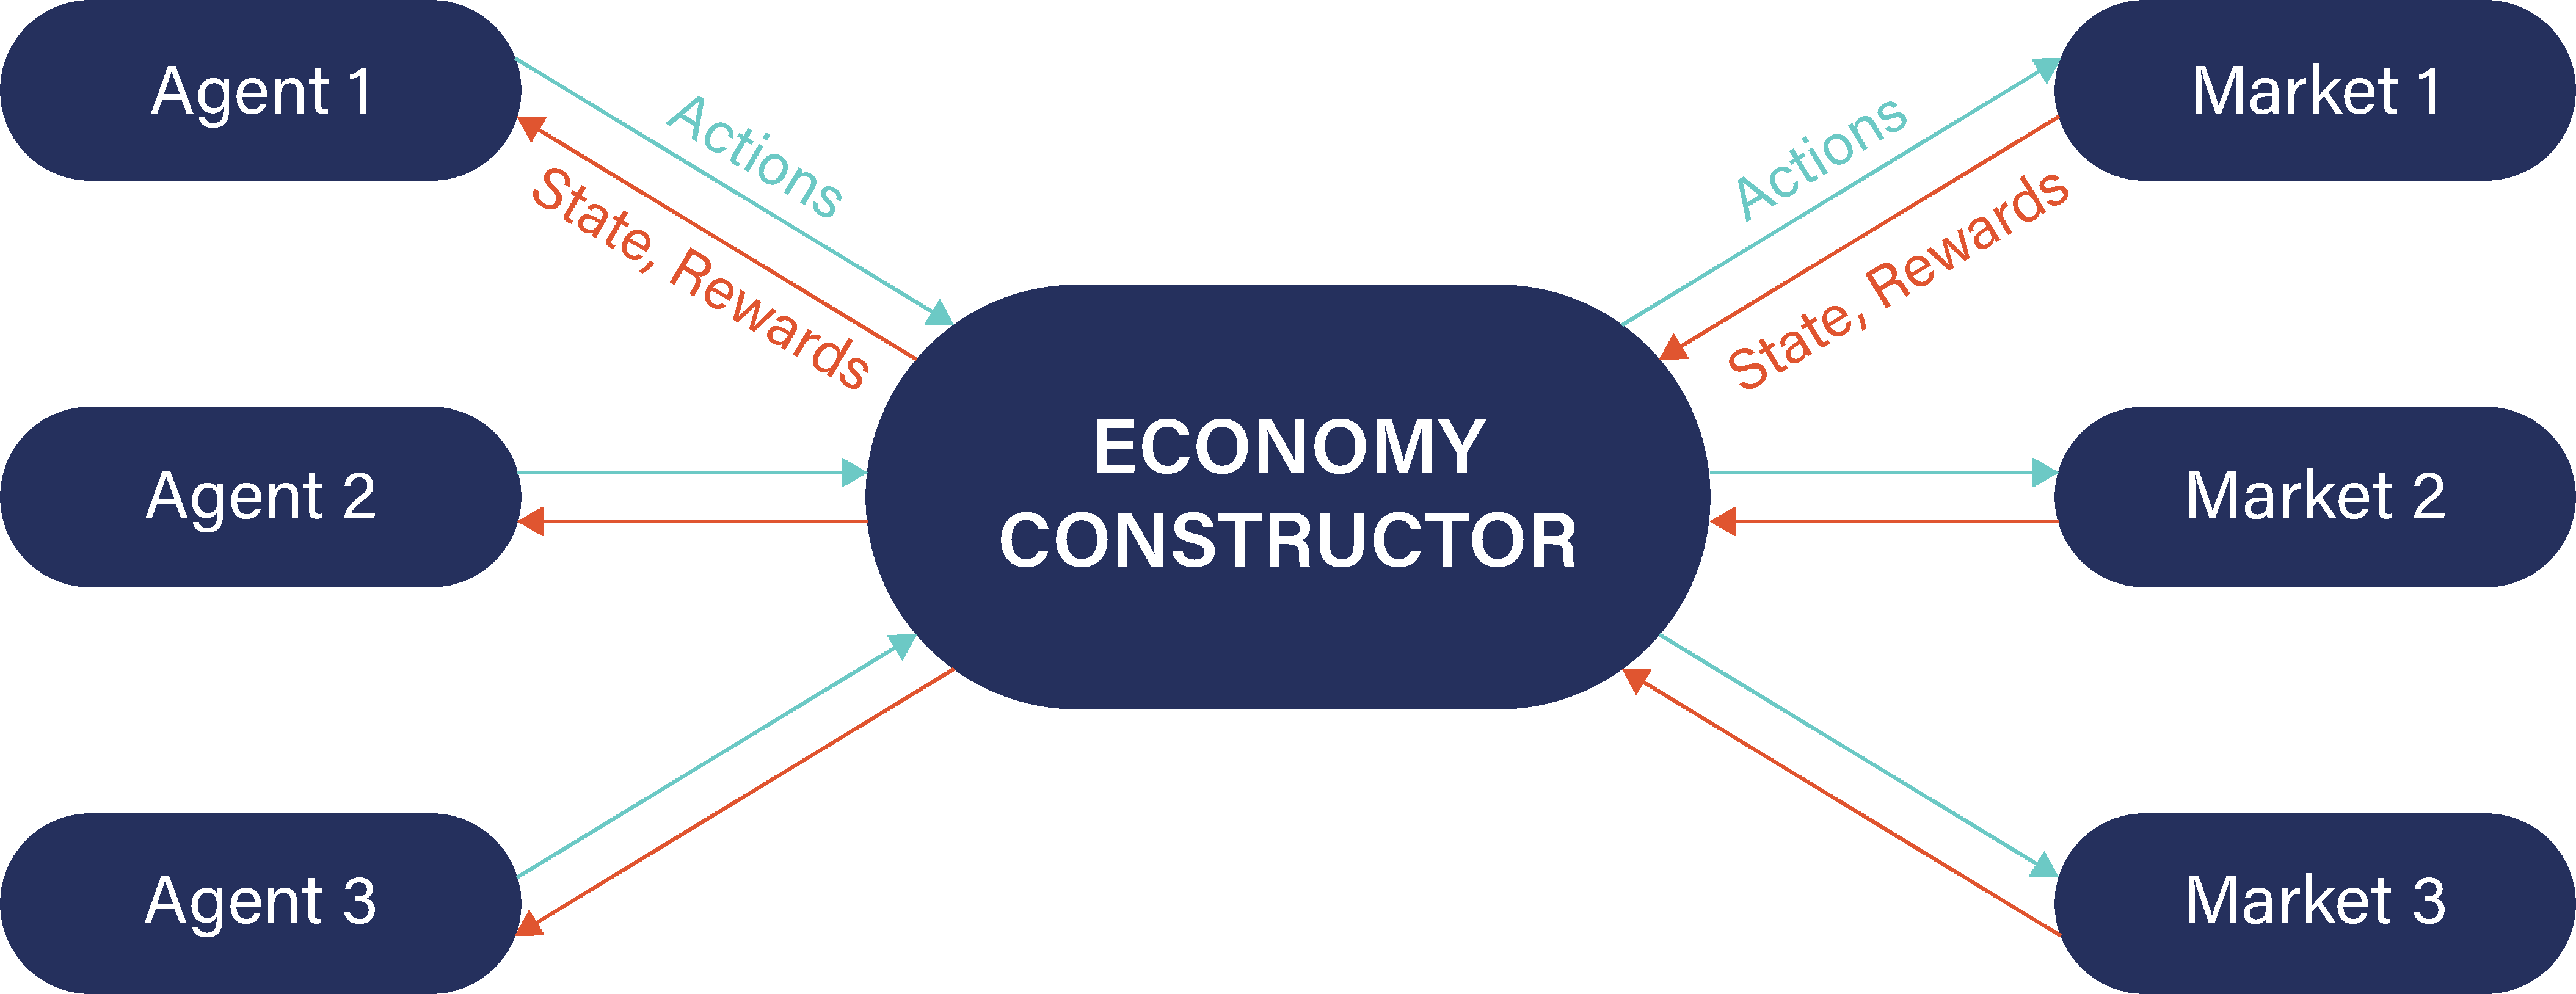
\includegraphics[scale=0.25]{\dir/econ_constructor.png}
\caption{Economic Constructor}
\end{figure}

\begin{itemize}
\item Three types of states: \ms
\begin{itemize}
\item Market specific states (e.g. prices, depreciation).
\item Agent specific states (e.g. productivity, preferences).
\item Economic specific states (e.g. aggregate productivity).
\end{itemize} 
\end{itemize}
\end{frame}

\begin{frame}
\frametitle{Customization of markets}

\begin{itemize}
	\item Both discrete and continuous action spaces are supported. \ms
	
	\item When declaring parameters, you can declare a stochastic process instead of a parameter. \ms
	\begin{itemize}
		\item e.g.:  \pyobject{substitution = iid\_Normal(coeffs=[0.15,0.1])} instead of \pyobject{substitution=0.15}. \ms
		\item The market automatically evaluates the stochastic function and includes i int market state. \ms
	\end{itemize}
	
	\item You can specify agents functional forms.\ms
	\begin{itemize}
		\item e.g.:  \pyobject{utility = CES(coeffs=1)}. \ms
	\end{itemize}
	
	\item If the market is created from an economy constructor, the market is automatically "Connected", which means that the imposing of budget constraints and registry of states is done at the economy level. \ms
	
	\item If the market is "Unconnected", it automatically imposes the budget constraints and keep registry of states.
	
\end{itemize}
\end{frame}

%%% SLIDE 13 %%%
\begin{frame}
\frametitle{Challenges to the framework}

\begin{enumerate}
	\item F.O.C.s are useful to introduce abstractions that simplify the environment. Example: Representative Agent. \ms
		\begin{itemize}
		\item A solution is to introduce F.O.C. based agents, which observe the state and solves their F.O.Cs each period. \ms
		\item In the extreme, we can specify the RL problem as one of submitting full equations (e.g. a demand schedule) and the environment act as auctioneer, solving for the equilibrium. \ms
	\end{itemize}
	
	\item Constraints do not have a natural implementation in the RL world. \ms
	\begin{itemize}
		\item A fast solution is to punish the agent if it violates a constraint during learning. \ms
		\item More complex solutions involve changing the action space as the environment evolves or adjusting the policy neural net so it always delivers an acceptable action. \ms
	\end{itemize}

	\item Non-stationarity of environment in early stages of learning might hinder progress. \ms
		\begin{itemize}
		\item A solution would be to use curriculum learning and abstract markets. \ms
		\item Agents may start playing against programed counterparts (as in diff. demand example) and then they start  learning against RL players. \ms
	\end{itemize}

\end{enumerate}

\end{frame}

\begin{frame}
\frametitle{Three possible Macro Avenues}

\begin{enumerate}
	\item Macro-financial model of Real Estate. \ms
	\begin{itemize}
		\item Start with Real Model, consisting of housing, CRE markets plus final (spot) market. Benchmark: Kydland and Prescott (1982).  \ms
		\item Add Intermediated Credit Market. Benchmark: Kaplan, Mitmal and Violante (2020) Elenev, Landvoight and Van Nieuwerburgh (2020).  \ms
		\item I can study macro effect of TTB or taxes.  \ms
	\end{itemize}
	
	\item Monetary Policy:  \ms
	\begin{itemize}
		\item Start with basic New Keynesian model with exogenous Taylor Rule.  \ms
		\item Add credit and banking. Benchmarks: Kaplan, Moll and Violante (2018).  \ms
		\item I can study equilibrium selection issues and test neo-fisherian hypothesis.  \ms
	\end{itemize}
	
	\item Incomplete Information:  \ms
	\begin{itemize}
		\item Start with basic Grossman and Stiglitz.  \ms
		\item Add real sector.   \ms
		\item I can study learning from prices in a dynamic setting.  \ms
	\end{itemize}
	
\end{enumerate}

\end{frame}

%%% SLIDE 13 %%%


\end{document} 